%\documentclass[9pt,xcolor={dvipsnames},handout]{beamer}
\documentclass[9pt,xcolor={dvipsnames}]{beamer}

\mode<presentation>{
  \usetheme{CambridgeUS}
  \usecolortheme{sysnove}
  \setbeamercovered{transparent}
}

\usepackage[french]{babel}
\usepackage[utf8]{inputenc}
\usepackage{times}
\usepackage[T1]{fontenc}
\usepackage[scaled=.95]{inconsolata}
\usepackage{graphics}
\usepackage{subfig}
\usepackage{multicol}
\usepackage{changepage}
\usepackage{marvosym}
\usepackage{eurosym}
\usepackage{amsmath}
%\usepackage{amssymb}
\usepackage[Q=yes]{examplep}
\usepackage{tcolorbox}
\tcbuselibrary{skins, xparse, listings, raster, breakable}
\usepackage{listings}
\usepackage{tikz}
\usetikzlibrary{babel, calc, tikzmark}

% Garphics path
\graphicspath{{imgs/}}

% General document information
\title[Outils de travail collaboratif]{{\small ADSILLH}\\Outils de travail collaboratif}
\author[Alexis Lahouze]{Alexis~\textsc{Lahouze}\\
  \medskip
  
\includegraphics[scale=0.5]{logo-sysnove}
}
\institute[Sysnove]{}
\date{ADSILLH 2016 S1}

% Color definitions
\setbeamerfont{author in sidebar}{size=\footnotesize}
\setbeamerfont{title in sidebar}{size=\footnotesize}
\setbeamerfont{subsection in sidebar}{size=\scriptsize}
\setbeamercolor{palette sidebar secondary}{fg=darkred}
\setbeamercolor{title in sidebar}{fg=darkred}

% Logo definition
\logo{
  
\includegraphics[height=0.6cm]{logo-sysnove}
  \hspace{0.5cm}
}

% Disable Beamer navigation bar
\setbeamertemplate{navigation symbols}{}
% Hide next entries when using \pause
%\setbeamercovered{invisible}

% Command to get the current section name
\usepackage{nameref}
\makeatletter
\newcommand*{\currentname}{\@currentlabelname}
\makeatother

% Automatically insert frame with current section summary
\AtBeginSection[]
{
  \begin{frame}{\currentname}
    \tableofcontents[
      currentsection,
      sectionstyle=show/shaded,
      subsectionstyle=show/show/hide
    ]
  \end{frame}
}

% Automatically insert frame with current section summary
\AtBeginSubsection[]
{
  \begin{frame}{\currentname}
    \tableofcontents[
      currentsection,
      sectionstyle=show/shaded,
      subsectionstyle=show/shaded/hide
    ]
  \end{frame}
}

% Define normal diff language for listings
\lstdefinelanguage[normal]{diff}{
  morecomment=[f][\color{BrickRed}]<,         % deleted lines 
  morecomment=[f][\color{ForestGreen}]>,      % added lines
}

% Define context diff for listings
\lstdefinelanguage[context]{diff}{
  morecomment=[f][\textbf]{!},                      % modified lines
  morecomment=[f][\color{BrickRed}]-,               % deleted lines 
  morecomment=[f][\color{ForestGreen}]+,            % added lines
  morecomment=[f][\color{BrickRed}]{***},    % original file information
  morecomment=[f][\color{ForestGreen}]{---}, % modified file information
  morecomment=[f][\color{black}]{***************},  % hunk separator
}

% Define unified diff for listings
\lstdefinelanguage[unified]{diff}{
  morecomment=[f][\color{blue}]{@@},          % group identifier
  morecomment=[f][\color{BrickRed}]-,         % deleted lines 
  morecomment=[f][\color{ForestGreen}]+,      % added lines
  morecomment=[f][\color{BrickRed}]{---},     % original file
  morecomment=[f][\color{ForestGreen}]{+++},  % modified file
}

% Basic listing style
\lstset{
  style=tcblatex,
  basicstyle=\tiny\ttfamily,
  numberstyle=\Tiny\ttfamily,
  numbers=left,
}

% Define some base styles. Blankest has been copied from tcolorbox v2016.
\tcbset{
  blankest/.style={blanker, notitle, frame hidden,
    no shadow, no underlay, no overlay, no finish, no borderline},
  snvbase/.style={beamer, colback=red0!10!white,
    colframe=red0!75!black, fonttitle=\tiny},
}
  
% Global listing declaration
\NewTCBListing{snvlisting}{ O{{}} m O{} O{} }{%
  snvbase,
  title=#2,
  lowerbox=ignored,
  listing only,
  listing options={language={#1}, #4},
  #3}%
    
\NewTCBInputListing{\snvinputlisting}{ O{{}} m m O{} O{} }{%
  snvbase,
  title=#2,
  lowerbox=ignored,
  left skip=-10pt,
  listing only,
  listing file=#3,
  listing options={language={#1}, #5},
  #4}%

% TColorBox listing for shell.
\NewTCBListing{shell}{ O{} O{\#} }{%
  snvbase,
  listing only,
  every listing line={\bfseries {#2}\ },
  listing options={language=sh},
  #1}%

% Finally the document
\begin{document}

% Title frame
\begin{frame}[plain]
  \titlepage
\end{frame}

% Main table of contents
\begin{frame}[squeeze]{Sommaire}
  \tableofcontents[sectionstyle=show, subsectionstyle=show/show/show]
\end{frame}

\section{Introduction}
\begin{frame}{Alexis Lahouze}
  \framesubtitle{Vie professsionnelle}

  \begin{itemize}
    \item 2001-2003~: IUT Informatique Bayonne
    \pause
    \item 2004-2011~: Capgemini~: dev Java et adminsys
    \pause
    \item 2011-2013~: F-Secure~: adminsys
    \pause
    \item 2013-~: Sysnove~: cofondateur
  \end{itemize}
\end{frame}

\begin{frame}{Alexis Lahouze}
  \framesubtitle{Contributions dans le libre}

  \begin{itemize}
    \item ABUL
    \pause
    \item RMLL
    \pause
    \item Relecteur LinuxFR
    \pause
    \item root lautre.net
    \pause
    \item Diverses contributions à des projets
  \end{itemize}
\end{frame}

\begin{frame}{Objectif}
  \framesubtitle{Contribuer}

  \begin{itemize}
    \item Comprendre les contraintes du travail en équipe\dots
    \pause
    \item \dots et à distance~;
    \pause
    \item Avoir un aperçu des outils utilisés dans les projets libres~;
    \pause
    \item Savoir partager son travail~;
    \pause
    \item Intégrer une communauté dans le cadre du projet tuteuré.
  \end{itemize}
\end{frame}

\section{Outils de Développement}

\subsection{Patch}

\begin{frame}{Premiers patchs}
 \begin{figure}
   \caption{Programme sur bande perforée patchée pour Harvard Mark I.}
   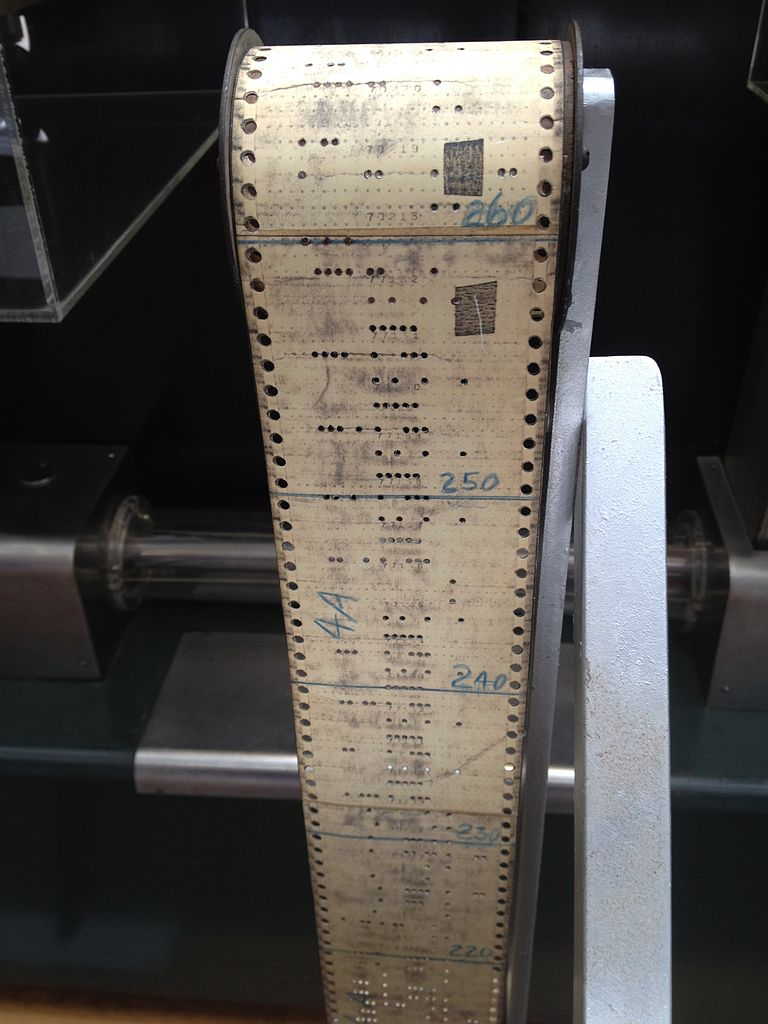
\includegraphics[height=160pt]{Harvard_Mark_I_program_tape}\par
   \tiny Source~: Wikipedia
 \end{figure}
\end{frame}

\begin{frame}[fragile]{Principe de base}
\begin{itemize}[<+->]
 \item Généralité~:
 \begin{itemize}
     \item Mécanisme permettant de modifier (correction, amélioration) une ressource.
  \end{itemize}
 \item Programmation~:
 \begin{itemize}[<+->]
    \item Fichier texte décrivant les différences entre deux fichiers texte~;
    \item Permet de stocker des incréments de modifications d'un fichier (révisions)~;
    \item Base de la gestion de versions.
  \end{itemize}
 \end{itemize}
\end{frame}

\begin{frame}[fragile]{Ligne de commande~: diff}
  \begin{itemize}[<+->]
  \item Commande de base permettant de comparer deux fichiers~:
  \begin{shell}
diff original.txt modifie.txt
  \end{shell}
  \item Series de ``morceaux'' (hunks)
  \begin{itemize}[<+->]
   \item Entête~: plages de lignes impactées et action~: \verb\ww[,yy]aWW[,YY]\~;
     \begin{description}[align=left]
      \item[a] add
      \pause
      \item[d] delete
      \pause
      \item[c] change (add and delete)
     \end{description}
   \item Lignes supprimées préfixées par \verb\<\~;
   \item Lignes ajoutées préfixées par \verb\>\~;
   \item Séparateur lorsque qu'il y a les deux (change)~: \verb\---\~;
   \item Dans le cas de plusieurs fichiers (\verb\-r\), la commande diff du fichier courant est ajoutée avant le premier morceau~: \verb\diff -r v1/fichier.txt v2/fichier.txt\~;
  \end{itemize}
  \item Possibilité d'avoir de la couleur avec \verb\colordiff\.
 \end{itemize}
\end{frame}

\begin{frame}[fragile]{Sortie normale de diff}
  \begin{tcbraster}[raster columns=3, raster valign=top]
  \begin{snvlisting}{original.txt}
This part of the
document has stayed the
same from version to
version.  It shouldn't
be shown if it doesn't
change.  Otherwise, that
would not be helping to
compress the size of the
changes.

This paragraph contains
text that is outdated.
It will be deleted in the
near future.

It is important to spell
check this dokument. On
the other hand, a
misspelled word isn't
the end of the world.
Nothing in the rest of
this paragraph needs to
be changed. Things can
be added after it.
  \end{snvlisting}
  \begin{snvlisting}{modifie.txt}
This is an important
notice! It should
therefore be located at
the beginning of this
document!

This part of the
document has stayed the
same from version to
version.  It shouldn't
be shown if it doesn't
change.  Otherwise, that
would not be helping to
compress anything.

It is important to spell
check this document. On
the other hand, a
misspelled word isn't
the end of the world.
Nothing in the rest of
this paragraph needs to
be changed. Things can
be added after it.

This paragraph contains
important new additions
to this document.
  \end{snvlisting}
  \begin{snvlisting}[[normal]diff]{diff original.txt modifie.txt}
0a1,6
> This is an important
> notice! It should
> therefore be located at
> the beginning of this
> document!
>
8,14c14
< compress the size of the
< changes.
<
< This paragraph contains
< text that is outdated.
< It will be deleted in the
< near future.
---
> compress anything.
17c17
< check this dokument. On
---
> check this document. On
24a25,28
>
> This paragraph contains
> important new additions
> to this document.
\end{snvlisting}
\end{tcbraster}
\end{frame}

\begin{frame}[fragile]{Script ed}
Format interprétable (presque) directement par la commande ed~:
\begin{shell}
printf "w\\nq\\n" >> v1v2.diff
ed -s original.txt < v1v2.diff
\end{shell}

\end{frame}

\begin{frame}[fragile]{Script ed}
\begin{tcbraster}[raster columns=3, raster valign=top]
  \begin{snvlisting}{original.txt}
This part of the
document has stayed the
same from version to
version.  It shouldn't
be shown if it doesn't
change.  Otherwise, that
would not be helping to
compress the size of the
changes.

This paragraph contains
text that is outdated.
It will be deleted in the
near future.

It is important to spell
check this dokument. On
the other hand, a
misspelled word isn't
the end of the world.
Nothing in the rest of
this paragraph needs to
be changed. Things can
be added after it.
  \end{snvlisting}
  \begin{snvlisting}{modifie.txt}
This is an important
notice! It should
therefore be located at
the beginning of this
document!

This part of the
document has stayed the
same from version to
version.  It shouldn't
be shown if it doesn't
change.  Otherwise, that
would not be helping to
compress anything.

It is important to spell
check this document. On
the other hand, a
misspelled word isn't
the end of the world.
Nothing in the rest of
this paragraph needs to
be changed. Things can
be added after it.

This paragraph contains
important new additions
to this document.
\end{snvlisting}
\begin{snvlisting}{diff -e original.txt modifie.txt}
24a

This paragraph contains
important new additions
to this document.
.
17c
check this document. On
.
8,14c
compress anything.
.
0a
This is an important
notice! It should
therefore be located at
the beginning of this
document!

.
\end{snvlisting}
\end{tcbraster}
\end{frame}

\begin{frame}[fragile]{Format contextuel}
\begin{itemize}[<+->]
 \item BSD 2.8 (Juillet 1981)~;
 \item Noms de fichiers et timestamp~;
 \item Lignes contexte~:
 \begin{itemize}[<+->]
  \item Lignes inchangées~;
  \item Préfixées par \textvisiblespace~;
  \item 3 par défaut~;
  \item Servent de référence pour valider la consistance du patch~;
  \item Permettent parfois de trouver l'emplacement du hunk lorsque les numéros de lignes sont changés dans le fichier sur lequel on applique le patch (fuzzy matching)~;
  \item Si lignes de contexte partagées entre deux parties modifiées, ces parties sont regroupées en un seul morceau.
 \end{itemize}
 \item Pas d'actions explicites, juste les préfixes \verb|-| (suppression), \verb|!| (modification) et \verb|+| (ajout)~;
 \end{itemize}
\end{frame}
 
\begin{frame}[fragile]{Format contextuel}
 \framesubtitle{Format d'un morceau}
 \begin{itemize}[<+->]
  \item Début~: \verb|***************|~;
  \item Plage de lignes concernées fichier source, encadrée par \verb|***|~;
  \item Contexte du début du morceau source, si pas au début du fichier~;
  \item Lignes supprimées (préfixées par \verb|-|), ou modifiées (préfixées par \verb|!|)~;
  \item Contexte de fin du morceau source, si pas en fin de fichier~;
  \item Plage de lignes concernées fichier cible, encadrée par \verb|---|~;
  \item Contexte du début du morceau cible, si pas au début du fichier~;
  \item Lignes ajoutées (préfixées par \verb|+|), ou modifiées (préfixées par \verb|!|)~;
  \item Contexte de fin du morceau cible, si pas en fin de fichier~;
 \end{itemize}
\end{frame}

\begin{frame}[fragile]{Format contextuel}
\begin{tcbraster}[raster columns=3, raster valign=top]
  \begin{snvlisting}{original.txt}
This part of the
document has stayed the
same from version to
version.  It shouldn't
be shown if it doesn't
change.  Otherwise, that
would not be helping to
compress the size of the
changes.

This paragraph contains
text that is outdated.
It will be deleted in the
near future.

It is important to spell
check this dokument. On
the other hand, a
misspelled word isn't
the end of the world.
Nothing in the rest of
this paragraph needs to
be changed. Things can
be added after it.
  \end{snvlisting}
  \begin{snvlisting}{modifie.txt}
This is an important
notice! It should
therefore be located at
the beginning of this
document!

This part of the
document has stayed the
same from version to
version.  It shouldn't
be shown if it doesn't
change.  Otherwise, that
would not be helping to
compress anything.

It is important to spell
check this document. On
the other hand, a
misspelled word isn't
the end of the world.
Nothing in the rest of
this paragraph needs to
be changed. Things can
be added after it.

This paragraph contains
important new additions
to this document.
\end{snvlisting}
\begin{snvlisting}[[context]diff]{diff -c original.txt modifie.txt}
*** original.txt	timestamp
--- modifie.txt	timestamp
***************
*** 1,3 ****
--- 1,9 ----
+ This is an important
+ notice! It should
+ therefore be located at
+ the beginning of this
+ document!
+
  This part of the
  document has stayed the
  same from version to
***************
*** 5,20 ****
  be shown if it doesn't
  change.  Otherwise, that
  would not be helping to
! compress the size of the
! changes.
!
! This paragraph contains
! text that is outdated.
! It will be deleted in the
! near future.

  It is important to spell
! check this dokument. On
  the other hand, a
  misspelled word isn't
  the end of the world.
--- 11,20 ----
  be shown if it doesn't
  change.  Otherwise, that
  would not be helping to
! compress anything.

  It is important to spell
! check this document. On
  the other hand, a
  misspelled word isn't
  the end of the world.
***************
*** 22,24 ****
--- 22,28 ----
  this paragraph needs to
  be changed. Things can
  be added after it.
+
+ This paragraph contains
+ important new additions
+ to this document.
\end{snvlisting}
\end{tcbraster}
\end{frame}

\begin{frame}[fragile]{Format unifié}
\begin{itemize}[<+->]
 \item Format développé en août 1990, ajouté à GNU diff 1.15 en janvier 1991~;
 \item Hérite des ajouts du format contextuel~:
 \begin{itemize}[<+->]
  \item Informations sur les fichiers~;
  \item Lignes de contexte.
 \end{itemize}
 \item Moins verbeux que le format contextuel car moins de répétitions~;
 \item Utilisé pour les échanges entre développeurs (notamment l'envoi par email).
\end{itemize}
\end{frame}

\begin{frame}[fragile]{Format unifié}
 \framesubtitle{Entête concernant le fichier impacté}
 \begin{itemize}[<+->]
  \item Fichier source préfixé par \verb|---| et timestamp de modification~;
  \item Fichier cible préfixé par \verb|+++| et timestamp de modification.
 \end{itemize}
\end{frame}

\begin{frame}[fragile]{Format unifié}
\framesubtitle{Format d'un morceau}
\begin{itemize}[<+->]
 \item Plages de lignes concernées~:
 \begin{itemize}[<+->]
   \item Chaque plage contient la ligne de début et la ligne de fin~;
   \item La plage côté source est préfixée par \verb|-|~;
   \item La plage côté cible est préfixée par \verb|+|~;
   \item Encadrées par \verb|@@|~;
   \item Optionnellement suivie d'un entête de section.
   \item \verb|@@ -l,s +l,s @@ optional section heading|
  \end{itemize}
  \item Contexte du début du morceau, si pas au début du fichier~;
  \item Lignes supprimées (préfixées par \verb|-|)~;
  \item Lignes ajoutées (préfixées par \verb|+|)~;
  \item Lignes modifiées : ajout et suppression~;
  \item Contexte de fin du morceau, si pas en fin de fichier~;
\end{itemize}
\end{frame}

\begin{frame}[fragile]{Format unifié}
\begin{tcbraster}[raster columns=3, raster valign=top, raster before skip=6pt]
  \begin{snvlisting}{original.txt}
This part of the
document has stayed the
same from version to
version.  It shouldn't
be shown if it doesn't
change.  Otherwise, that
would not be helping to
compress the size of the
changes.

This paragraph contains
text that is outdated.
It will be deleted in the
near future.

It is important to spell
check this dokument. On
the other hand, a
misspelled word isn't
the end of the world.
Nothing in the rest of
this paragraph needs to
be changed. Things can
be added after it.
  \end{snvlisting}
  \begin{snvlisting}{modifie.txt}
This is an important
notice! It should
therefore be located at
the beginning of this
document!

This part of the
document has stayed the
same from version to
version.  It shouldn't
be shown if it doesn't
change.  Otherwise, that
would not be helping to
compress anything.

It is important to spell
check this document. On
the other hand, a
misspelled word isn't
the end of the world.
Nothing in the rest of
this paragraph needs to
be changed. Things can
be added after it.

This paragraph contains
important new additions
to this document.
\end{snvlisting}
\begin{snvlisting}[[unified]diff]{diff -u original.txt modifie.txt}
--- original.txt   timestamp
+++ modifie.txt   timestamp
@@ -1,3 +1,9 @@
+This is an important
+notice! It should
+therefore be located at
+the beginning of this
+document!
+
 This part of the
 document has stayed the
 same from version to
@@ -5,16 +11,10 @@
 be shown if it doesn't
 change.  Otherwise, that
 would not be helping to
-compress the size of the
-changes.
-
-This paragraph contains
-text that is outdated.
-It will be deleted in the
-near future.
+compress anything.

 It is important to spell
-check this dokument. On
+check this document. On
 the other hand, a
 misspelled word isn't
 the end of the world.
@@ -22,3 +22,7 @@
 this paragraph needs to
 be changed. Things can
 be added after it.
+
+This paragraph contains
+important new additions
+to this document.
\end{snvlisting}
\end{tcbraster}
\end{frame}

\begin{frame}[fragile]{Application d'un patch}
\framesubtitle{Commande patch}
\begin{itemize}[<+->]
 \item Première version publié en 1985~:
 \begin{itemize}[<+->]
 \item Sur newsgroup \verb/mod.sources/ (devenu \verb/comp.sources.unix/)~;
 \item Par Larry Wall (créateur de Perl).
 \end{itemize}
 \item Version la plus utilisée~: GNU.
\end{itemize}
\end{frame}

\begin{frame}[fragile]{Commande patch}
\framesubtitle{Invocation}
 \begin{shell}
patch < v1v2.diff
 \end{shell}

 \begin{itemize}[<+->]
 \item Essaie de détecter le format parmis normal, script ed, contextuel ou unifié~;
 \item Se sert des informations de fichiers et de lignes dans le patch~;
 \item Si le patch n'est pas applicable directement, tente d'ignorer un certain nombre de lignes des contextes (fuzz factor, 2 par défaut)~;
 \item En cas de non application d'un morceau, il le met dans un fichier de rejet dont le nom est celui du fichier impacté suffixé par \verb|.rej|.
 \end{itemize}
\end{frame}
 
\begin{frame}[fragile]{Commande patch}
\framesubtitle{Options utiles}
\begin{itemize}[<+->]
 \item Forcer le format du patch~:
 \begin{itemize}[<+->]
  \item Normal~: \verb/-n/ ou \verb/--normal/~;
  \item Script ed~: \verb/-e/ ou \verb/--ed/~;
  \item Contextuel~: \verb/-c/ ou \verb/--context/~;
  \item Unifié~: \verb/-u/ ou \verb/--unified/.
 \end{itemize}
 \item Répertoire de travail~: \verb/-d/ ou \verb/--directory/~;
 \item Tronquer le début des chemins~: \verb/-p/num ou \verb/--strip=/num~: \verb/patch -p1 < v1v2.diff/
 \item Application inverse d'un patch (reverse, ou rollback)~: \verb/-R/ ou \verb/--reverse/~: \verb/patch -R < v1v2.diff/~;
 \item Suppression des fichiers vides après application du patch~: \verb/-E/ ou \verb/--remove-empty-files/~;
 \item Sauvegarde des fichiers originaux~: \verb/-b/ ou \verb/--backup/~;
% \item Mode bavard~: \verb/--verbose/.
\end{itemize}
\end{frame}

\begin{frame}[fragile]{Commande patch}
\framesubtitle{Exemples d'invocation}
\begin{tcbraster}[raster columns=2, raster valign=top]
\begin{snvlisting}[[unified]diff]{v1v2.diff}
diff -u v1/f1.txt v2/f1.txt
--- v1/f1.txt   2016-09-09 16:06:41.632285371 +0200
+++ v2/f1.txt   2016-09-09 16:07:12.913211867 +0200
@@ -1,3 +1,9 @@
+This is an important
+notice! It should
+therefore be located at
+the beginning of this
+document!
+
 This part of the
 document has stayed the
 same from version to
@@ -5,16 +11,10 @@
 be shown if it doesn't
 change.  Otherwise, that
 would not be helping to
-compress the size of the
-changes.
-
-This paragraph contains
-text that is outdated.
-It will be deleted in the
-near future.
+compress anything.

 It is important to spell
-check this dokument. On
+check this document. On
 the other hand, a
 misspelled word isn't
 the end of the world.
\end{snvlisting}
\begin{snvlisting}[[unified]diff]{}
@@ -22,3 +22,7 @@
 this paragraph needs to
 be changed. Things can
 be added after it.
+
+This paragraph contains
+important new additions
+to this document.
\end{snvlisting}
\end{tcbraster}
\end{frame}

\begin{frame}[fragile]{Commande patch}
\framesubtitle{Exemples d'invocation}
\begin{tcbraster}[raster columns=2, raster valign=top]
\begin{snvlisting}{Application réussie d'un patch}[][escapeinside={}]
# patch --verbose -p1 < v1v2.diff
Hmm...  Looks like a unified diff to me...
The text leading up to this was:
--------------------------
|diff -du v1/f1.txt v2/f1.txt
|--- v1/f1.txt  2016-09-11 16:06:41.632285371 +0200
|+++ v2/f1.txt  2016-09-11 16:07:12.913211867 +0200
--------------------------
patching file f1.txt
Using Plan A...
Hunk #1 succeeded at 1.
Hunk #2 succeeded at 11.
Hunk #3 succeeded at 22.
done
\end{snvlisting}
\begin{snvlisting}{Application échouée d'un patch}[][escapeinside={}]
# patch --verbose -p1 < v1v2.diff
Hmm...  Looks like a unified diff to me...
The text leading up to this was:
--------------------------
|diff -du v1/f1.txt v2/f1.txt
|--- v1/f1.txt  2016-09-11 16:06:41.632285371 +0200
|+++ v2/f1.txt  2016-09-11 16:07:12.913211867 +0200
--------------------------
patching file f1.txt
Using Plan A...
Reversed (or previously applied) patch detected!  Assume -R? [n] n
Apply anyway? [n] y
Hunk #1 FAILED at 1.
Hunk #2 FAILED at 5.
Hunk #3 FAILED at 22.
3 out of 3 hunks FAILED -- saving rejects to file f1.txt.rej
done
\end{snvlisting}
\end{tcbraster}
\end{frame}

\begin{frame}[fragile]{Commande patch}
\framesubtitle{Exemples d'invocation}
\begin{tcbraster}[raster columns=2, raster valign=top]
\begin{snvlisting}[[unified]diff]{f1.txt.rej}
--- f1.txt      2016-09-11 16:06:41.632285371 +0200
+++ f1.txt      2016-09-11 16:07:12.913211867 +0200
@@ -1,3 +1,9 @@
+This is an important
+notice! It should
+therefore be located at
+the beginning of this
+document!
+
 This part of the
 document has stayed the
 same from version to
@@ -5,16 +11,10 @@
 be shown if it doesn't
 change.  Otherwise, that
 would not be helping to
-compress the size of the
-changes.
-
-This paragraph contains
-text that is outdated.
-It will be deleted in the
-near future.
+compress anything.

 It is important to spell
-check this dokument. On
+check this document. On
 the other hand, a
 misspelled word isn't
 the end of the world.
\end{snvlisting}
\begin{snvlisting}[[unified]diff]{}
@@ -22,3 +22,7 @@
 this paragraph needs to
 be changed. Things can
 be added after it.
+
+This paragraph contains
+important new additions
+to this document.
\end{snvlisting}
\end{tcbraster}
\end{frame}

\begin{frame}[fragile]{Commande patch}
\framesubtitle{Exemples d'invocation}
 \begin{snvlisting}[[normal]diff]{diff ../v1v2.diff f1.txt.rej}
1,3c1,2
< diff -du v1/f1.txt v2/f1.txt
< --- v1/f1.txt 2016-09-11 16:06:41.632285371 +0200
< +++ v2/f1.txt 2016-09-11 16:07:12.913211867 +0200
---
> --- f1.txt    2016-09-11 16:06:41.632285371 +0200
> +++ f1.txt    2016-09-11 16:07:12.913211867 +0200
 \end{snvlisting}
\end{frame}

\begin{frame}[fragile]{Autres outils}
\framesubtitle{Merges avec diff3}
\begin{tcbraster}[raster columns=3, raster valign=top]
\begin{snvlisting}{diff3 -m v3/f1.txt v1/f1.txt v2/f1.txt}[][escapeinside={}]
This is an important
notice! It should
therefore be located at
the beginning of this
document!

This part of the
document has stayed the
same from version to
version.  It shouldn't
be shown if it doesn't
change.  Otherwise, that
would not be helping to
\end{snvlisting}
\begin{snvlisting}{}[][escapeinside={}]
<<<<<<< v3/f1.txt
compress the size of the
changes.

This paragraph contains
text that has been
modified on both sides.
It will be deleted in the
near future.
||||||| v1/f1.txt
compress the size of the
changes.

This paragraph contains
text that is outdated.
It will be deleted in the
near future.
=======
compress anything.
>>>>>>> v2/f1.txt
\end{snvlisting}
\begin{snvlisting}{}[][escapeinside={}]

It is important to spell
check this document. On
the other hand, a
misspelled word isn't
the end of the world.
Nothing in the rest of
this paragraph needs to
be changed. Things can
be added after it.

This paragraph contains
important new additions
to this document.
\end{snvlisting}
\end{tcbraster}
\end{frame}

\begin{frame}[fragile]{Autres outils}
\framesubtitle{Quilt}
\begin{itemize}[<+->]
 \item Nommé d'après patchwork quilt (courtepointe en patchwork)~;
 \item Permet de regrouper des ensembles de patchs en un seul~;
 \item Initialement développé par Andrew Morton, développeur Kernel Linux~;
 \item \url{https://stuff.mit.edu/afs/athena/system/i386_deb50/os/usr/share/doc/quilt/quilt.html}~;
 \item Très utilisé dans les projets Linux et Debian~;
 \item \url{https://wiki.debian.org/UsingQuilt}.
\end{itemize}
\end{frame}

%\begin{frame}{Cas pratiques}
%\framesubtitle{Paquet Debian : linux-image}
%\end{frame}

\subsection{Gestion du code source}

\begin{frame}{Systèmes de gestion de versions}
\begin{itemize}[<+->]
 \item Local~:
 \begin{itemize}[<+->]
  \item SCCS~: remplacé par~:
  \item RCS~: remplacé par~:
 \end{itemize}
 \item Client-serveur~:
 \begin{itemize}[<+->]
  \item Tous ceux utilisés actuellement.
 \end{itemize}
 \item Deux modes principaux~:
 \begin{itemize}
 \item Centralisé
 \item Décentralisé
 \end{itemize}
\end{itemize}
\end{frame}

\begin{frame}{Systèmes de gestion de versions centralisés}
\begin{itemize}[<+->]
 \item Principe~:
 \begin{itemize}
  \item Chaque modification (commit) est envoyée directement sur le serveur.
 \end{itemize}
 \item Les plus connus~:
 \begin{itemize}[<+->]
  \item CVS
  \item Subversion
 \end{itemize}
 \item Inconvénient~: Nécessite une connexion pour envoyer ses modifications.
\end{itemize}
\end{frame}

\begin{frame}{Systèmes de gestion de versions décentralisés}
\begin{itemize}[<+->]
 \item Principe~:
 \begin{itemize}
  \item Chaque modification (commit) est stockée localement.
  \item L'ensemble des modifications est envoyée à un dépôt distant (remote)~;
  \item Possibilité d'avoir plusieurs dépôts distants.
 \end{itemize}
 \item Les plus connus~:
 \begin{itemize}[<+->]
  \item BitKeeper
  \item Git
  \item Mercurial
  \item GNU Bazaar (successeur de GNU Arch)
 \end{itemize}
 \item Avantage~: Pas besoin de connexion pour commiter~;
 \item Inconvénient~: Workflow plus complexe.
\end{itemize}
\end{frame}

\begin{frame}{Lexique}
\begin{description}[align=left]
 \item [Trunk] version de développement principale~;
 \begin{itemize}[<+->]
  \item Très instable~;
  \item Version à partir de laquelle on crée les branches et les tags~;
  \item Appelé aussi 'master' (Git).
 \end{itemize}
 \pause
 \item [Tags] version figée (release)~;
 \begin{itemize}[<+->]
  \item Ne doit pas être modifié directement\dots
  \item \dots donc utilisation de branches de maintenance.
 \end{itemize}
 \pause
 \item [Branche] version de développement secondaire~;
 \begin{itemize}[<+->]
  \item Branche de maintenance de version (hotfix)~;
  \item Branche de fonctionnalité (feature).
 \end{itemize}
 \pause
 \item [Révision/commit] modification atomique d'un ou plusieurs fichiers~;
 \pause
 \item [Head] dernière révision du dépôt~;
 \pause
 \item [Objet] élément versionnable (fichier, répertoire, lien symbolique, etc.).
\end{description}
\end{frame}

\begin{frame}{Utilisation générale}
\framesubtitle{Que faut-il versionner~?}
\begin{itemize}[<+->]
 \item Tout ce qui est susceptible d'être modifié au cours du temps~:
 \begin{itemize}[<+->]
  \item Code source~;
  \item Script de construction~;
  \item Documentation.
 \end{itemize}
 \item Mais pas ce qui est générable~:
 \begin{itemize}[<+->]
  \item Code compilé~;
  \item Documentation d'API~;
  \item Etc.~;
  \item Les différents systèmes possèdent un mécanisme d'ignore.
 \end{itemize}
\end{itemize}
\end{frame}

\begin{frame}{Utilisation générale}
\framesubtitle{Quand faut-il commiter~?}
\begin{itemize}[<+->]
 \item Le plus souvent possible~;
 \item Quand ça marche~:
 \begin{itemize}[<+->]
  \item Compile sans erreur~;
  \item Testé et validé.
 \end{itemize}
 \item Un commit inclut une modification et une seule.
 \begin{itemize}[<+->]
  \item Éviter les commits monolythiques.
 \end{itemize}
\end{itemize}
\end{frame}

\begin{frame}[fragile]{Subversion}
\framesubtitle{Informations générales}
\begin{itemize}[<+->]
 \item Anciens développeurs de CVS~;
 \item Première version en 2000\dots
 \item \dots version 1.0.0 en 2004~;
 \item Dernière version~:1.9.5 (29 novembre 2016)~;
 \item Un dépôt central, sur un serveur, sur les protocoles~:
 \begin{itemize}[<+->]
  \item SVN (svnserve, TCP 3690)~;
  \item HTTP (webdav, passe dans plus d'infrastructures réseau).
 \end{itemize}
 \item Pas de notion de branche ou de tag, utilisation de l'arborescence~;
 \item Possibilité de checkout une sous-arborescence~;
 \item Numéros de versions séquentiels, globaux au dépôt~;
 \item Les répertoires sont versionnés (notamment les répertoires vides)~;
 \item \url{http://svnbook.red-bean.com/} (assez ancienne, mais toujours d'actualité).
\end{itemize}
\end{frame}

\begin{frame}{Subversion}
\framesubtitle{Architecture d'un dépôt}
  \begin{itemize}[<+->]
   \item trunk
   \begin{itemize}[<+->]
    \item Développements courants~;
   \end{itemize}
   \item branches
   \begin{itemize}[<+->]
    \item Développements conséquents~;
    \item Maintenances de versions~;
   \end{itemize}
   \item tags
   \begin{itemize}[<+->]
    \item Versions figées~;
    \item Pas de modification dans les tags~;
   \end{itemize}
 \end{itemize}
\end{frame}

\begin{frame}{Subversion}
\framesubtitle{Architecture d'un dépôt}
 \begin{figure}
   \caption{Worflow de développement avec Subversion.}
   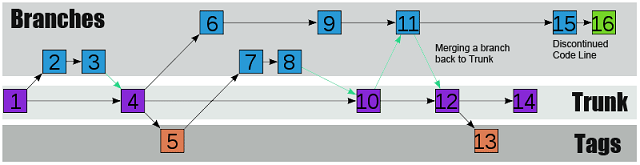
\includegraphics[width=345pt]{repository-structure3}\par
   \tiny Source~: \url{http://blogs.wandisco.com/2011/10/24/subversion-best-practices-repository-structure/}
 \end{figure}
\end{frame}

\begin{frame}{Subversion}
\framesubtitle{Workflow de développement}
\begin{description}
 \item [\Q{svn checkout}] créer sa copie locale~;
 \pause
 \item [\Q{svn update}] mettre à jour sa copie locale avec les modifications des autres~;
 \pause
 \item [\Q{svn add}] ajouter des fichiers~;
 \pause
 \item [\Q{svn copy}] copier des fichiers ou une sous-arborescence~;
 \begin{itemize}
  \item Sert particulièrement à créer les branches et les tags.
 \end{itemize}
 \pause
 \item [\Q{svn delete}] supprimer des fichiers~;
 \pause
 \item [\Q{svn move}] déplacer des fichies~;
 \pause
 \item [\Q{svn status}] voir l'état de la copie locale~;
 \pause
 \item [\Q{svn diff}] voir les différences entre deux versions, ou de sa copie locale par rapport à la dernière mise à jour du dépôt~;
 \pause
 \item [\Q{svn revert}] annuler une modification application inversée du diff d'un commit)~;
 \pause
 \item [\Q{svn resolve}] effectuer une gestion des conflits sur un fichier~;
 \pause
 \item [\Q{svn resolved}] marquer un conflit comme résolu~;
 \pause
 \item [\Q{svn commit}] pousser ses modifications sur le dépôt~;
 \pause
 \item [\Q{svn merge}] fusionner une branche dans une autre~;
 \pause
 \item [\Q{svn switch}] changer de branche (changer le point d'origine dans l'arborescence distante)~;
 \pause
 \item [\Q{svn info}] avoir les informations de sa copie locale.
\end{description}
\end{frame}

\begin{frame}[fragile]{Subversion}
\frametitle{svn status}
\begin{itemize}[<+->]
 \item Affiche l'état de la copie locale~;
 \item Permet d'avoir les modifications sur le serveur avec l'option \verb/--show-updates/ ou \verb/-u/~;
\end{itemize}
\begin{snvlisting}{Exemple d'invocation (honteusement copié sur \url{http://svnbook.red-bean.com/en/1.8/svn.ref.svn.c.status.html})}[][escapeinside={}]
# svn status -u wc
 M            965    wc/bar.c
        *     965    wc/foo.c
A  +          965    wc/qax.c
Status against revision:    981
\end{snvlisting}
\end{frame}

\begin{frame}[fragile]{Subversion}
\frametitle{svn status -- format}
\begin{itemize}[<+->]
 \item Première colonne~: changements sur l'objet~:
 \begin{description}[align=left]
  \item [\textvisiblespace] objet inchangé~;
  \item [A] objet ajouté (\verb/svn add/)~;
  \item [D] objet supprimé (\verb/svn delete/)~;
  \item [M] objet modifié~;
  \item [C] objet en conflit (après \verb/svn update/)~;
  \item [I] objet ignoré~;
  \item [?] objet inconnu (non ajouté)~;
  \item [!] objet manquant (supprimé du système de fichiers mais pas avec \verb/svn delete/)
  \item [\textasciitilde] objet ayant changé de type (par ex.~: fichier -> répertoire)
 \end{description}
\end{itemize}
\end{frame}

\begin{frame}[fragile]{Subversion}
\frametitle{svn status -- format}
\begin{itemize}[<+->]
 \item Seconde colonne~: changements sur les propriétés de l'objet~:
 \begin{description}[align=left]
  \item [\textvisiblespace] propriétés inchangées~;
  \item [M] propriétés modifiées~;
  \item [C] propriétés en conflit (modifiées localement et sur le dépôt distant).
 \end{description}
 \item Troisième colonne~: L si copie locale verrouillée~;
 \item Quatrième colonne~: + si ajout avec historique~;
 \item Cinquième colonne~: S si l'objet a changé de branche~;
 \item Sixième colonne~: informations de verrouillage distant~;
 \item Septième colonne~: informations de conflit d'arbre~;
 \item Huitième colonne~: toujours une espace~;
 \item Neuvième colonne~: * si l'objet est périmé (mis à jour sur le dépôt distant)~;
 \item Révision locale (si \verb/--show-updates/ ou \verb/--verbose/ passé en paramètre)~;
 \item Dernière révision commitée (si \verb/--verbose/ passé en paramètre)~;
 \item Toujours en dernier~: chemin de l'objet concerné, peut contenir des espaces.
\end{itemize}
\end{frame}

\begin{frame}[fragile]{Subversion}
\frametitle{svn info}
\begin{snvlisting}{Exemple d'invocation (honteusement copié sur \url{http://svnbook.red-bean.com/en/1.8/svn.ref.svn.c.info.html})}[][escapeinside={}]
# svn info foo.c
Path: foo.c
Name: foo.c
Working Copy Root Path: /home/sally/projects/test
URL: http://svn.red-bean.com/repos/test/foo.c
Repository Root: http://svn.red-bean.com/repos/test
Repository UUID: 5e7d134a-54fb-0310-bd04-b611643e5c25
Revision: 4417
Node Kind: file
Schedule: normal
Last Changed Author: sally
Last Changed Rev: 20
Last Changed Date: 2003-01-13 16:43:13 -0600 (Mon, 13 Jan 2003)
Text Last Updated: 2003-01-16 21:18:16 -0600 (Thu, 16 Jan 2003)
Properties Last Updated: 2003-01-13 21:50:19 -0600 (Mon, 13 Jan 2003)
Checksum: d6aeb60b0662ccceb6bce4bac344cb66
\end{snvlisting}
\end{frame}

\begin{frame}[fragile]{Subversion}
\frametitle{Propriétés}
\begin{itemize}[<+->]
 \item Métadonnées des objets~;
 \item Clé-valeur~;
 \item Personnalisées ou réservées à subversion (préfixées par \verb/svn:/)
 \item Commandes~:
 \begin{description}
  \item [\Q{svn proplist <objet>}] affiche les propriétés d'un objet~;
  \item [\Q{svn propedit <nom> <objet>}] ouvre un éditeur pour définir la valeur d'une propriété d'un objet~;
  \item [\Q{svn propset <nom> <valeur> <objet>}] définit la valeur d'une propriété d'un objet~;
  \item [\Q{svn propdel <nom> <objet>}] supprime la propriété de l'objet.
 \end{description}
 \item Quelques propriétés connues~:
 \begin{description}
  \item [\Q{svn:ignore}] liste des objets non versionnés~;
  \item [\Q{svn:eol-style}] type de fin de ligne (unix, dos)~;
  \item [\Q{svn:author}] auteur de la révision~;
  \item [\Q{svn:date}] date de la révision~;
  \item [\Q{svn:log}] message de révision.
 \end{description}
\end{itemize}
\end{frame}

\begin{frame}[fragile]{Subversion}
\frametitle{\Q{svn:ignore}}
\begin{itemize}[<+->]
 \item Contient la liste des patterns d'objets ignorés~;
 \item S'applique à un répertoire.
\end{itemize}
\begin{snvlisting}{Exemple}[][escapeinside={}]
*~
.*.sw*
*.pyc
\end{snvlisting}
\end{frame}

\begin{frame}{Subversion}
 \framesubtitle{Outils annexes}
 \begin{description}
  \item [TortoiseSVN] Intégration dans l'explorateur de fichiers Windows~;
  \pause
  \item [eSVN] Interface graphique dédiée, multiplateforme~;
  \pause
  \item [kdesvn] Interface graphique dédiée, Linux uniquement~;
  \pause
  \item [Différents IDE] La plupart des IDE ont une intégration de subversion~;
  \pause
  \item [Forges] Outils web intégrés pour le développement.
  \pause
  \item [Etc.] Modules d'éditeurs de texte, intégration gestionnaires de fichiers, \dots
  \pause
 \end{description}
\end{frame}

\begin{frame}[fragile]{Git}
\frametitle{Informations générales}
\begin{itemize}[<+->]
 \item Initialement écrit par Linus Torvalds pour remplacer BitKeeper~;
 \item Première version le 7 avril 2005~;
 \item Dernière version le 4 août 2017 (2.14.1)~;
 \item Possibilité d'avoir plusieurs dépôts distants (remote)~;
 \item Accessibles via les protocoles~:
 \begin{itemize}
  \item SSH (authentification par clé)
  \item HTTP (clonage anonyme)
  \item git (en pratique peu utilisé)
 \end{itemize}
 \item La copie locale est un clone (complet ou incomplet) du dépôt distant~;
 \item Notions de tags et de branches~;
 \item Pas de séquence, utilisation de hash pour identifier les commits~;
 \item Les répertoires ne sont pas versionnés, donc absence de répertoires vides~;
 \item Possibilité d'étendre la commande (\verb/git flow/ par exemple)~;
 \item \url{https://git-scm.com/book/fr/v2/}.
\end{itemize}
\end{frame}

\begin{frame}{Git}
\framesubtitle{Terminologie}
\begin{description}
 \item [blob] contenu d'un objet versionné (fichier)~;
 \pause
 \item [commit] révision, hash et commit parent~;
 \pause
 \item [branche] version active du projet~;
 \pause
 \item [tag] étiquette sur un point donné de l'historique, permet de figer des releases~;
 \pause
 \item [merge] fusion entre deux branches~;
 \pause
 \item [rebase] changement de la base de la branche par une autre branche~;
 \pause
 \item [staging] aussi appelé cache, contient les objets et états servant au commit~;
 \pause
 \item [stash] pile dans laquelle le développeur peut stocker ses modifications sans les commiter, souvent avant un pull pour fusionner ses modifications a posteriori.
\end{description}
\end{frame}

\begin{frame}{Git}
\framesubtitle{Workflow}
\begin{description}
 \item [\Q{git clone}] clone un dépôt distant en local~;
 \pause
 \item [édition] modifie les fichiers~;
 \pause
 \item [\Q{git stash}] sauvegarde les modifications dans stash~;
 \pause
 \item [\Q{git pull}] récupére les révisions distantes~;
 \pause
 \item [\Q{git stash pop}] réapplique les modifications sur la copie de travail à jour~;
 \pause
 \item [\Q{git mergetool}] lance l'outil de gestion des conflits (lors d'un pull, ou d'un merge)~;
 \pause
 \item [\Q{git add}] ajoute un fichier modifié ou non versionné dans le cache~;
 \pause
 \item [\Q{git rm}] supprime un fichier et le met comme tel dans le cache~;
 \pause
 \item [\Q{git commit}] crée une révision locale d'après le cache~;
 \pause
 \item [\Q{git push}] pousse les révisions locales~;
\end{description}
\end{frame}
 
\begin{frame}{Git}
\framesubtitle{Workflow -- suite}
\begin{description}
 \item [\Q{git branch}] manipule les branches~;
 \pause
 \item [\Q{git checkout}] change de branche, ou restaure un fichier de travail~;
 \pause
 \item [\Q{git reset}] réinitialise HEAD à un état différent~;
 \pause
 \item [\Q{git merge}] fusionne une branche dans la branche courante~;
 \pause
 \item [\Q{git mergetool}] lance l'outil de gestion des conflits si nécessaire~;
 \pause
 \item [\Q{git rebase}] reconstruit l'historique de la branche par rapport à une autre branche~;
 \pause
 \item [\Q{git tag}] manipule les tags, possibilité de le signe avec une clé PGP.
\end{description}
\end{frame}

\begin{frame}[fragile]{Git}
\frametitle{Autres commandes utiles}
\begin{description}
 \pause
 \item [\Q{git blame}] affiche le commit et l'auteur de chaque ligne d'un fichier~;
 \pause
 \item [\Q{git diff}] affiche les différences sur la copie locale, ou entre deux révisions~;
 \begin{itemize}[<+->]
  \item Permet de générer un fichier patch, avec l'option \verb/--patch/ ou \verb/-p/ ou encore \verb/-u/~;
 \end{itemize}
 \pause
 \item [\Q{git submodule}] gère les sous-modules~;
 \pause
 \item [\Q{git help <command>}] RTFM ;-) Attention, très (trop) complet.
\end{description}
\end{frame}

\begin{frame}{Git}
 \frametitle{Workflow simple}
 \begin{figure}
   \caption{Worflow de développement local avec Git.}
   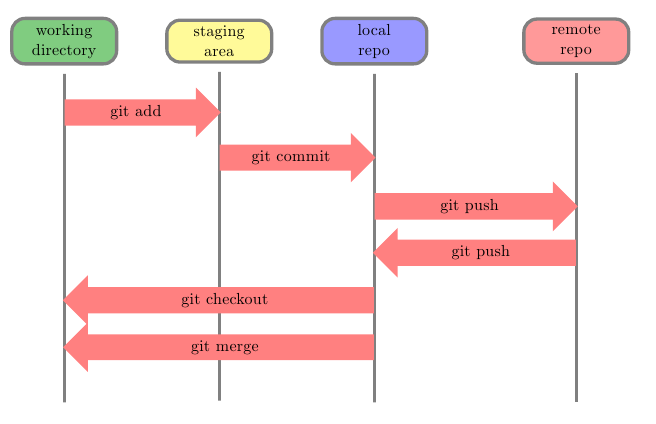
\includegraphics[height=160pt]{git-base-workflow}\par
   \tiny Source~: \url{http://tex.stackexchange.com/questions/70320/workflow-diagram}
 \end{figure}
\end{frame}

\begin{frame}[fragile]{Git}
\frametitle{\Q{git status}}
\begin{snvlisting}{Exemple}[][escapeinside=||]
On branch master
Your branch is up-to-date with 'origin/master'.
Changes to be committed:
  (use "git reset HEAD <file>..." to unstage)

        modified:   mailcap

Changes not staged for commit:
  (use "git add <file>..." to update what will be committed)
  (use "git checkout -- <file>..." to discard changes in working directory)

        modified:   caffrc
        modified:   config/i3pystatus/config.py
        modified:   dotfilesrc
        modified:   mutt-profiles/alexis@lahouze.org/profile
        modified:   mutt-profiles/alexis@sysnove.fr/profile
        modified:   offlineimaprc
        modified:   services/dunst/log/run
        modified:   tmux.conf
        modified:   vimrc
        modified:   zshrc

Untracked files:
  (use "git add <file>..." to include in what will be committed)

        config/flexget/
        imapnotify.js

\end{snvlisting}
\end{frame}

\begin{frame}[fragile]{Git}
\frametitle{Sous-modules}
\begin{itemize}[<+->]
 \item Référence de dépôts git dans des sous-répertoires du dépôt~;
 \item Ne se mettent pas à jour automatiquement~;
 \item Enregistré dans \verb/.gitmodules/~;
 \item Workflow~:
 \begin{itemize}[<+->]
  \item \verb/git submodule add/
  \item \verb/git commit -m "..."/
  \item \verb/git submodule update/
 \end{itemize}
 \item \url{https://git-scm.com/book/fr/v1/Utilitaires-Git-Sous-modules}
\end{itemize}
\end{frame}

\begin{frame}[fragile]{Git}
 \frametitle{Git Flow}
 \begin{itemize}[<+->]
  \item Décrit par Vincent Driesse sur \url{http://nvie.com/posts/a-successful-git-branching-model/}
  \item Process de développement et de publication standardisé~;
  \item Commande \verb/git flow/ (\url{https://github.com/nvie/gitflow}).
  \item Antisèche~: \url{http://danielkummer.github.io/git-flow-cheatsheet/}
 \end{itemize}
\end{frame}

\begin{frame}[fragile]{Git}
 \frametitle{Git Flow}
 \begin{figure}
   \caption{Workflow complet avec git flow.}
   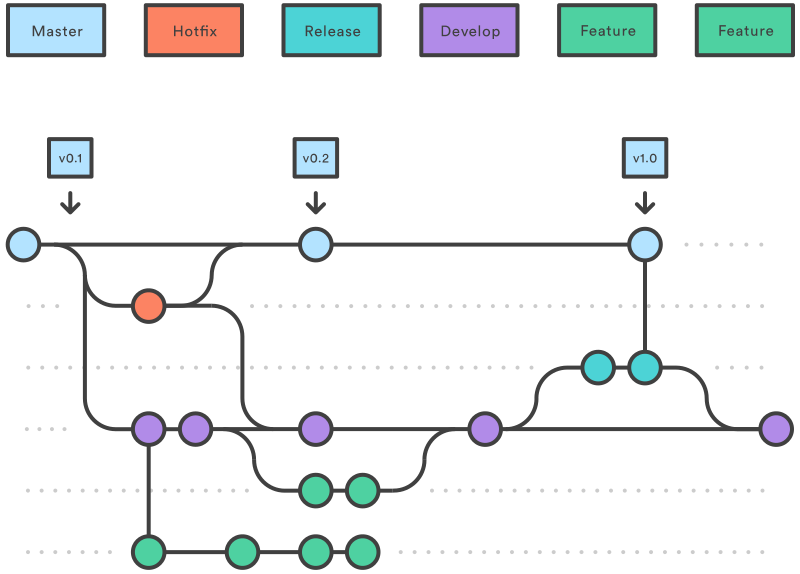
\includegraphics[height=160pt]{Gitflow-workflow}\par
   \tiny Source~: \url{https://www.atlassian.com/git/tutorials/comparing-workflows/gitflow-workflow}
 \end{figure}
\end{frame}

\begin{frame}[fragile]{Git}
\frametitle{git svn}
\begin{itemize}[<+->]
 \item Possibilité pour Git de se connecter à un dépôt Subversion~;
 \item Permet d'effectuer des commits locaux~;
 \item Ne permet pas de décentraliser le développement.
 \item \url{https://git-scm.com/book/fr/v2/Git-et-les-autres-systèmes-Git-comme-client#Git-et-Subversion}
\end{itemize}
\end{frame}

\begin{frame}[fragile]{Git}
\frametitle{git svn -- utilisation de base}
\begin{description}
 \item [\Q{git svn clone}] équivalent à \verb/svn checkout/~;
 \pause
 \item [\Q{git add}, \Q{git commit}] travailler localement~;
 \pause
 \item [\Q{git svn rebase}] équivalent à \verb/svn update/~;
 \pause
 \item [\Q{git svn dcommit}] équivalent à \verb/svn commit/ pour chaque commit local~;
 \pause
 \item [\Q{git svn branch}] manipule les branches et les tags (\verb/--tag/ ou \verb/--t/)~;
 \pause
 \item [\Q{git svn log}] affiche l'historique~;
 \pause
 \item [\Q{git svn blame}] affiche l'auteur et la révision de chaque ligne d'un fichier~;
 \pause
 \item [\Q{git svn reset}] permet de revenir à une révision spécifique~;
 \pause
 \item [\Q{git svn help}] RTFM ;-)
\end{description}
\end{frame}

\begin{frame}[fragile]{Git}
 \frametitle{Exemples - Cas simple}
 \begin{itemize}[<+->]
  \item Créer un dépôt sur Github
  \item Configurer son git local (user, email)
  \item Initialiser la copie locale
  \item Ignorer les fichiers constructibles, temporaires, etc.
  \item Ajouter les fichiers nécessaires au projet
  \item Commiter la branche \verb/master/
  \item Créer une branche \verb/develop/ et basculer dessus
  \item Ajouter un fichier README
  \item Ajouter dans le cache
  \item Commiter
  \item Modifier un fichier
  \item Ajouter dans le cache
  \item Commiter
  \item Merger dans \verb/master/
 \end{itemize}

\end{frame}


\section{Gestion de la Documentation}

\begin{frame}[fragile]{Outils}
\begin{description}
 \item [Wiki] Utilisé surtout pour la documentation technique~;
 \pause
 \item [Pad] Édition collaborative de texte (Etherpad)~:
 \begin{itemize}
  \pause
  \item Utilisés souvent pour des travaux ponctuels~;
  \pause
  \item \url{https://framapad.org}~;
  \pause
  \item \url{https://pad.ilico.org}~:
 \end{itemize}
 \pause
 \item [Cloud] Synchronisation, partage de fichiers, parfois édition en ligne (NextCloud, Cozy coud)~:
 \begin{itemize}
  \pause
  \item Autohébergés la plupart du temps~;
  \pause
  \item \url{https://framadrive.org}~;
  \pause
  \item Google Drive, MS Onedrive, etc. (non libres).
 \end{itemize}
\end{description}
\end{frame}



\section{Outils de Communication}

\subsection{Notions générales}

\begin{frame}[fragile]{Netiquette}
\begin{itemize}[<+->]
 \item Règles de bonne conduite sur les Internets
 \item Network Etiquette
 \item RFC1855~: \url{http://fgouget.free.fr/netiquette/rfc1855-fr.html}
 \item Communications un à un (mail, messagerie instantanée)
 \item Communications un à plusieurs (listes de diffusion, forums)
 \item Forme
 \begin{itemize}[<+->]
  \item Écrire en entier (pas de langage SMS)~;
  \item Écrire en minuscules, ÉCRIRE EN MAJUSCULES REVIENT À CRIER~;
  \item Réponses sous questions~;
  \item Ne pas dépasser 65 charactères dans un mail~;
  \item Etc.
 \end{itemize}
 \item Fond
 \begin{itemize}[<+->]
  \item Politesse
  \item Respect
 \end{itemize}
\end{itemize}
\end{frame}

\begin{frame}{Types de communication}
 \begin{itemize}[<+->]
  \item Interne~:
  \begin{itemize}[<+->]
   \item Entre les membres du projets, et les contributeurs~;
   \item Liés à l'évolution du projet.
  \end{itemize}
  \item Externe/publique~:
  \begin{itemize}
   \item Nouvelles du projet (versions, évolutions importantes).
  \end{itemize}
 \end{itemize}
\end{frame}

\begin{frame}{Modes de communication}
 \begin{itemize}[<+->]
  \item Synchrones (messagerie instantanée)
  \begin{itemize}[<+->]
   \item IRC
   \item ICQ
   \item Aol Instant Messaging
   \item MSN Messenger
   \item XMPP
   \item VoIP
  \end{itemize}
  \item Asynchrones
  \begin{itemize}[<+->]
   \item Usenet/Newsgroups
   \item Mail
   \item Forums
  \end{itemize}
 \end{itemize}
\end{frame}

\subsection{Communication synchrone}

\begin{frame}[fragile]{Internet Relay Chat}
\framesubtitle{Informations générales}
\begin{itemize}[<+->]
 \item RFC 1459 (août 1988), puis RFC 2810 à 2813 (2000)~;
 \item Client-Serveur~;
 \item Réseaux (plusieurs serveurs connectés entre eux)~;
 \item Discussion orientée salon de discussion (canal, channel, chan)~;
 \item \url{\#canal@reseau}~;
 \item \url{utilisateur@reseau}~;
 \item Modes utilisateur : Opérateur du réseau (o), invisible (i), \dots
 \item Modes~: Opérateur (o), voice (v), Secret (s), \dots
 \item Canal et pseudos volatiles.
\end{itemize}
\end{frame}

\begin{frame}[fragile]{Internet Relay Chat}
\framesubtitle{Réseaux connus}
\begin{itemize}[<+->]
 \item IRCnet~: \url{http://www.ircnet.org}
 \item DALnet~: \url{http://www.dal.net}
 \item EFnet~: \url{http://www.efnet.org}
 \item Undernet~: \url{http://www.undernet.org}
 \item QuakeNet~: \url{http://www.quakenet.org}
 \item Freenode~: \url{http://www.freenode.org}
 \begin{itemize}[<+->]
  \item Alexis Lahouze~: xals
  \item Samuel Thibault~: youpi
  \item Cyril Roelandt~: Steap
  \item \url{\#aquilenet}
  \item \url{\#adsillh}
  \item \url{\#abul}
 \end{itemize}
 \item Geeknode~: \url{http://www.geeknode.org}
 \begin{itemize}[<+->]
  \item Alexis Lahouze~: xals
  \item Samuel Thibault~: youpi
  \item Cyril Roelandt~: Steap
  \item \url{\#fdn}
  \item \url{\#sysnove}
 \end{itemize}
 \item OFTC (Debian)~: \url{http://www.oftc.net}
 \begin{itemize}[<+->]
  \item \url{\#debian-fr}
 \end{itemize}
\end{itemize}
\end{frame}

\begin{frame}{Internet Relay Chat}
\framesubtitle{Bots}
\begin{itemize}
  \item À l'origine créés pour éviter une prise de contrôle par quelqu'un d'autre (takeover) d'un canal ou d'un pseudo en cas d'absence~;
  \pause
  \item Permettent de transférer des informations sur le canal~;
  \pause
  \item Peuvent réagir à des mots (commandes)~;
  \pause
  \item La plupart des réseaux ont leur propre bot de gestion~:
  \begin{itemize}
   \pause
   \item Freenode~: ChanServ et NickServ
   \pause
   \item Geeknode~: C
  \end{itemize}

  \pause
  \item Quelques logiciels de bot connus~:
  \begin{itemize}
   \pause
   \item Supybot~;
   \pause
   \item Hubot~;
   \pause
   \item Eggdrop~;
   \pause
   \item Etc.
  \end{itemize}
 \end{itemize}
\end{frame}
 
\begin{frame}{Internet Relay Chat}
\framesubtitle{Clients les plus connus}
\begin{itemize}
 \item Console~:
 \begin{itemize}
  \item BitchX (semble maintenu car derniers commits dans la journée, mais dernière release le 14 novembre 2014)
  \pause
  \item Irssi (toujours actif, dernière release le 21 septembre dernier)
  \pause
  \item Weechat (très actif)
 \end{itemize}
 \pause
 \item Graphiques~:
 \begin{itemize}
  \item mIRC (Windows, développement toujours actif)~;
  \pause
  \item kvIRC (multiplateforme, anciennement KDE)~;
  \pause
  \item konversation (KDE)~;
  \pause
  \item XChat (GTK)~;
  \pause
  \item Chatzilla (extension Firefox)~;
  \pause
  \item Pidgin (GTK)~;
  \pause
  \item Passerelles XMPP <-> IRC.
 \end{itemize}
\end{itemize}
\end{frame}

\begin{frame}{XMPP (Jabber)}
\framesubtitle{Informations générales}
\begin{itemize}
 \item Créé en 1998, standardisé IETF en 2002 (RFC 3920 à 3923)~;
 \pause
 \item Client-Serveur-Serveur (interconnexion des domaines)~;
 \pause
 \item Orienté discussion un à un (comme ICQ)~;
 \pause
 \item Liste de contacts~;
 \pause
 \item Chiffrage bout en bout avec OTR et PGP.
\end{itemize}
\end{frame}

\begin{frame}{XMPP (Jabber)}
\framesubtitle{Logiciels Clients}
\begin{itemize}
 \item Pidgin (multiplateforme)
 \pause
 \item Gajim (multiplateforme)
 \pause
 \item Psi (multiplateforme)
 \pause
 \item Xabber (Android)
 \pause
 \item Conversations (Android)
 \pause
 \item Kopete (Linux, multiprotocole)
 \pause
 \item Miranda IM (Windows, multiprotocole)
 \pause
 \item Jappix (Web/Ajax)
 \pause
 \item Bitlbee (Linux, serveur IRC, client multiprotocole)
 \pause
 \item Etc.
\end{itemize}
\end{frame}

\begin{frame}{XMPP (Jabber)}
\framesubtitle{Logiciels Serveurs}
\begin{itemize}
 \item Jabberd14 (C)~;
 \pause
 \item Jabberd2 (C)~;
 \pause
 \item eJabberd (erlang)~;
 \pause
 \item Prosody (Lua)~;
 \pause
 \item Tigase (Java)~;
 \pause
 \item Etc.
\end{itemize}
\end{frame}

\begin{frame}{XMPP (Jabber)}
\framesubtitle{Services XMPP connus}
\begin{itemize}
 \item GTalk (Google)
 \pause
 \item im.apinc.org (FR)
 \pause
 \item jabber.im
\end{itemize}

\end{frame}

\begin{frame}{Autres systèmes}
\begin{itemize}
 \item La plupart propriétaires~;
 \pause
 \item Slack~;
 \begin{itemize}
  \item Notion d'équipes~;
  \pause
  \item Possibilité de connecter des applications externes~;
  \pause
  \item Utilisé par les startups.
 \end{itemize}
 \pause
 \item Gitter (github)~;
 \begin{itemize}
  \item Orienté projet.
 \end{itemize}
 \pause
 \item Certains réseaux sociaux~;
 \pause
 \item Etc.
\end{itemize}
\end{frame}

\subsection{Communication asynchrone}

\begin{frame}{Notion de base}
 \begin{itemize}
  \item On sait quand ça part, mais on ne sait pas quand ça arrive.
 \end{itemize}
\end{frame}

\begin{frame}{Usenet/Newsgroups}
\begin{itemize}
 \item Inventé en 1979~;
 \pause
 \item Client-serveur~;
 \pause
 \item Protocole UUCP (Unix to Unix Copy Protocol) puis NNTP (Network News Transfer Protocol)~;
 \pause
 \item Réseau de forums~;
 \pause
 \item Génération, stockage et récupération d'articles~;
 \pause
 \item Très proche du mail~;
 \pause
 \item Notion de groupes et d'abonnements à ces groupes.
\end{itemize}
\end{frame}

\begin{frame}[fragile]{Mails}
\framesubtitle{Informations générales}
\begin{itemize}
 \item Prémisses en 1965~;
 \pause
 \item RFC 561 en 1971, puis RFC 680, 724 et enfin 733 en 1977~: entêtes et protocole~;
 \pause
 \item RFC 822 en 1982~: format des messages~;
 \pause
 \item RFC 2045 à 2049~: MIME~;
 \pause
 \item RFC 2822 en 2001~: remplace la 822~;
 \pause
 \item RFC 5322 en 2008~: étend la 2822~;
 \pause
 \item Client-Serveur-Serveur~;
 \pause
 \item Chiffrage avec PGP (clé asymétrique), ou S/MIME (certificat numérique)~;
 \pause
 \item Organisation par sujets (threads)~:
 \begin{itemize}
  \pause
  \item Entête \verb/In-Reply-To/.
 \end{itemize}
\end{itemize}
\end{frame}

\begin{frame}{Mails}
\framesubtitle{Mailing-lists}
\begin{itemize}
 \item Mails gérés par un robot de liste, ou gestionnaire de listes~;
 \pause
 \item Le gestionnaire permet de gérer les abonnements~;
 \pause
 \item Adresse de destination unique~;
 \pause
 \item Redirection à tous les abonnés~;
 \pause
 \item Utilisées pour communiquer entre les membres de l'équipe~;
 \pause
 \item Utilisées pour communiquer avec l'extérieur (newsletters)~;
 \pause
 \item Souvent couplées à une interface web de gestion~;
 \pause
 \item Archives~;
 \pause
 \item Aggrégateurs de listes publiques~:
 \begin{itemize}
 \pause
  \item \url{http://www.gmane.org} (listes de diffusion et newsgroups)~;
 \end{itemize}

 \pause
 \item Moteurs connus~:
 \begin{itemize}
  \pause
  \item Sympa
  \pause
  \item Mailman
  \pause
  \item Majordomo
 \end{itemize}
\end{itemize}
\end{frame}

\begin{frame}{Mails}
\framesubtitle{Mailing-lists, entêtes spécifiques}
\begin{description}
 \item RFC 4021~;
 \pause
 \item [List-ID] Identifiant de la liste, permet une classification~;
 \pause
 \item [List-Owner] Adresse du propriétaire de la liste~;
 \pause
 \item [List-Post] Adresse d'envoi de la liste~;
 \pause
 \item [List-Subscribe] Adresse d'abonnement à la liste~;
 \pause
 \item [List-Unsubscribe] Adresse de désabonnement de la liste~;
 \pause
 \item [List-Help] Adresse pour obtenir de l'aide sur la liste~;
 \pause
 \item [List-Archive] Adresse de l'archive de la liste.
\end{description}
\end{frame}

\begin{frame}[fragile]{Forum}
\begin{itemize}[<+->]
 \item Site web~;
 \pause
 \item Hierachie~: Catégories, Sujets, Messages~;
 \pause
 \item Souvent des passerelles mails (envoi et gestion des réponses)~:
 \begin{itemize}[<+->]
  \item catégorie => mailing list~;
  \pause
  \item sujet => thread~;
  \pause
  \item message => mail.
 \end{itemize}
 \pause
 \item \url{https://www.hardware.fr}
\end{itemize}
\end{frame}

\begin{frame}{Bugtrackers}
\begin{itemize}
 \item Site web, mailing lists
 \pause
 \item Permet de recencer et suivre les tâches du projet
 \pause
 \item Anomalies (bugs) et fonctionnalités
 \pause
 \item Moteurs connus~:
 \begin{itemize}
  \item Bugzilla~;
  \pause
  \item Mantis~;
  \pause
  \item Flyspray~;
  \pause
  \item Debian BTS (emails, chaque bug est une liste de diffusion)~;
  \pause
  \item Forges.
 \end{itemize}
\end{itemize}
\end{frame}


\section{Forges de développement}

\begin{frame}{Informations générales}
\begin{itemize}
 \item Plateformes Web dédiées au développement~;
 \pause
 \item Intégration de différents outils~:
 \begin{itemize}
  \pause
  \item Site web dédié au projet~;
  \pause
  \item Gestionnaire de version~;
  \pause
  \item Bugtracker~;
  \pause
  \item Gestionnaire de documentation (wiki)~;
  \pause
  \item Listes de discussion, forums.
 \end{itemize}
\end{itemize}
\end{frame}

\begin{frame}{Logiciels (autohébergement)}
\begin{itemize}
 \item SourceForge et forks~:
  \pause
 \begin{itemize}
  \item FusionForge (ex-GForge)~;
  \pause
  \item Savane~;
  \pause
  \item Berlios~;
  \pause
  \item TeamForge (propriétaire).
 \end{itemize}
 \item Trac~;
  \pause
 \item Redmine/Chiliproject~;
  \pause
 \item Gitlab (double licence communauté et entreprise)~;
  \pause
 \item Gogs~;
  \pause
 \item Phabricator~;
  \pause
 \item Github (propriétaire).
\end{itemize}
\end{frame}

\begin{frame}[fragile]{Plateforme publiques}
\begin{itemize}
 \item \url{http://sourceforge.net}~: CVS, SVN, Git~;
 \pause
 \item \url{http://savannah.gnu.org}~: GNU Arch, GNU Bazaar, CVS, Git, Mercurial, Subversion~;
 \pause
 \item \url{http://gna.org}~: CVS, GNU Arch, Subversion~;
 \pause
 \item \url{http://github.com}~: Git~;
 \pause
 \item \url{http://gitlab.com} (ex Gitorious)~: Git.
 \pause
 \item \url{http://framagit.org} (Gitlab)
\end{itemize}
\end{frame}


\section{Fonctionnement de certains projets}

\begin{frame}[fragile]{Debian}
\begin{description}
 \item [Type] Distribution GNU/Linux~;
 \item [Site web] \url{https://www.debian.org}~;
 \item [IRC] OFTC~: \verb/#debian/ et \verb/#debian-fr/~;
 \item [Bugtracker] \url{https://www.debian.org/Bugs}, \url{mail://request@bugs.debian.org}~;
 \item [Mailing-lists] \url{https://lists.debian.org/}~:
 \begin{description}[align=left]
  \item [debian-announce] Informations capitales et changements importants dans le projet, modérée~;
  \item [debian-backports] Discussion sur les backports, non modérée~;
  \item [debian-user] Aide pour les utilisateurs de Debian, volume important, non modérée~;
  \item [debian-user-french] Aide francophone pour les utilisateurs de Debian~;
  \item Liste complète sur \url{https://www.debian.org/MailingLists/subscribe}.
 \end{description}
 \item [Forge] \url{https://alioth.debian.org} (GForge)
 \item [Contribution] \url{https://www.debian.org/devel/join/}
\end{description}
\end{frame}

\begin{frame}[fragile]{Linux}
 \begin{description}
  \item [Type] Noyau du système d'exploitation~;
  \item [Site web] \url{https://www.kernel.org}~;
  \item [Patchs] \url{https://patchwork.kernel.org}~;
  \item [Bugtracker] \url{https://bugzilla.kernel.org/}~;
  \item [Mailing-lists] \url{http://vger.kernel.org/}~;
  \item [Wikis] \url{https://www.wiki.kernel.org/}~;
  \item [Git] \url{https://git.kernel.org}.
 \end{description}
\end{frame}

\begin{frame}[fragile]{KDE}
 \begin{description}
  \item [Type] Gestionnaire de bureaux, applications bureautiques~;
  \item [Site Web] \url{https://www.kde.org}~;
  \item [Wiki utilisateurs] \url{https://userbase.kde.org}~;
  \item [Wiki admin] \url{https://techbase.kde.org}~;
  \item [Wiki communauté] \url{https://community.kde.org}~;
  \item [Forum] \url{https://forum.kde.org/}~;
  \item [Mailing lists] \url{https://www.kde.org/support/mailinglists/}
  \item [Bugtracker] \url{https://bugs.kde.org/}~;
  \item [Git] \url{https://community.kde.org/Infrastructure/Git}~;
  \item [Contribuer] \url{https://community.kde.org/Get_Involved}.
 \end{description}
\end{frame}


\end{document}
